%-----------------------------------------------------------------------------80
% SECTION TITLE
%-----------------------------------------------------------------------------80
\section{Entorno de desarrollo}


%-----------------------------------------------------------------------------80
% CONTENT
%-----------------------------------------------------------------------------80
% Definición -----------------------------------------------------------------80
\subsection{Introducción}

\begin{frame}[fragile]{Entorno de desarrollo}
  \begin{figure}
      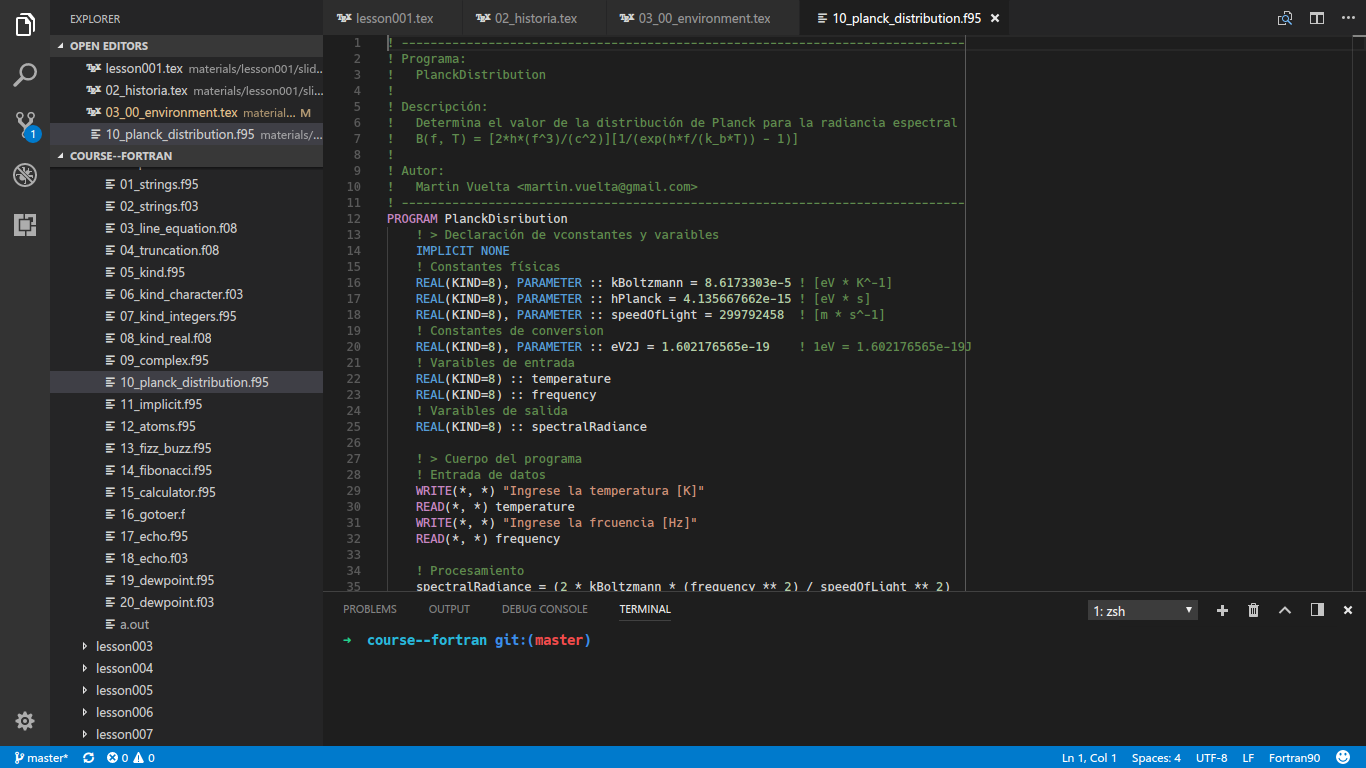
\includegraphics[width=1\textwidth]{./resources/IDE-VSCODE.png}
      \caption{Entorno de desarrollo VS Code}
  \end{figure}
\end{frame}

\begin{frame}[fragile]{Entorno de desarrollo}
  \textbf{Que tiene un entorno de desarrollo}
  \begin{itemize}[<+(1)->]
    \item Editor de código
    \item Compiladores o intérpretes
    \item Debugger
    \item Otras utilidades
  \end{itemize}
\end{frame}


\begin{frame}[fragile]{Entorno de desarrollo}
  \textbf{Editor de código}
  \begin{itemize}[<+(1)->]
    \item VS Code + Fortran Package [{\color{green-600}\faCheck}]
    \item Sublime Text
    \item Atom
    \item Vim
    \item Emacs
    \item ...
  \end{itemize}
\end{frame}
 

\begin{frame}[fragile]{Entorno de desarrollo}
  \textbf{Compilador}
  \begin{itemize}[<+(1)->]
    \item GFortran [{\color{green-600}\faCheck}]
    \item Intel
    \item IBM
    \item Oracle
    \item ...
  \end{itemize}
\end{frame}


\begin{frame}[fragile]{Entorno de desarrollo}
  \textbf{Debuggers}
  \begin{itemize}[<+(1)->]
    \item gdb [{\color{green-600}\faCheck}]
    \item idb
    \item ddd
    \item totalview
    \item ...
  \end{itemize}
\end{frame}
